%!TEX root = ../NCVC2.tex

\mysection{形状認識処理}

\subsection{CADデータの読み込み}
 とりあえず普通にCADデータを開いてください.
ここではサンプルの maizuru.jww を開きます.

\begin{figure}[H]
\centering
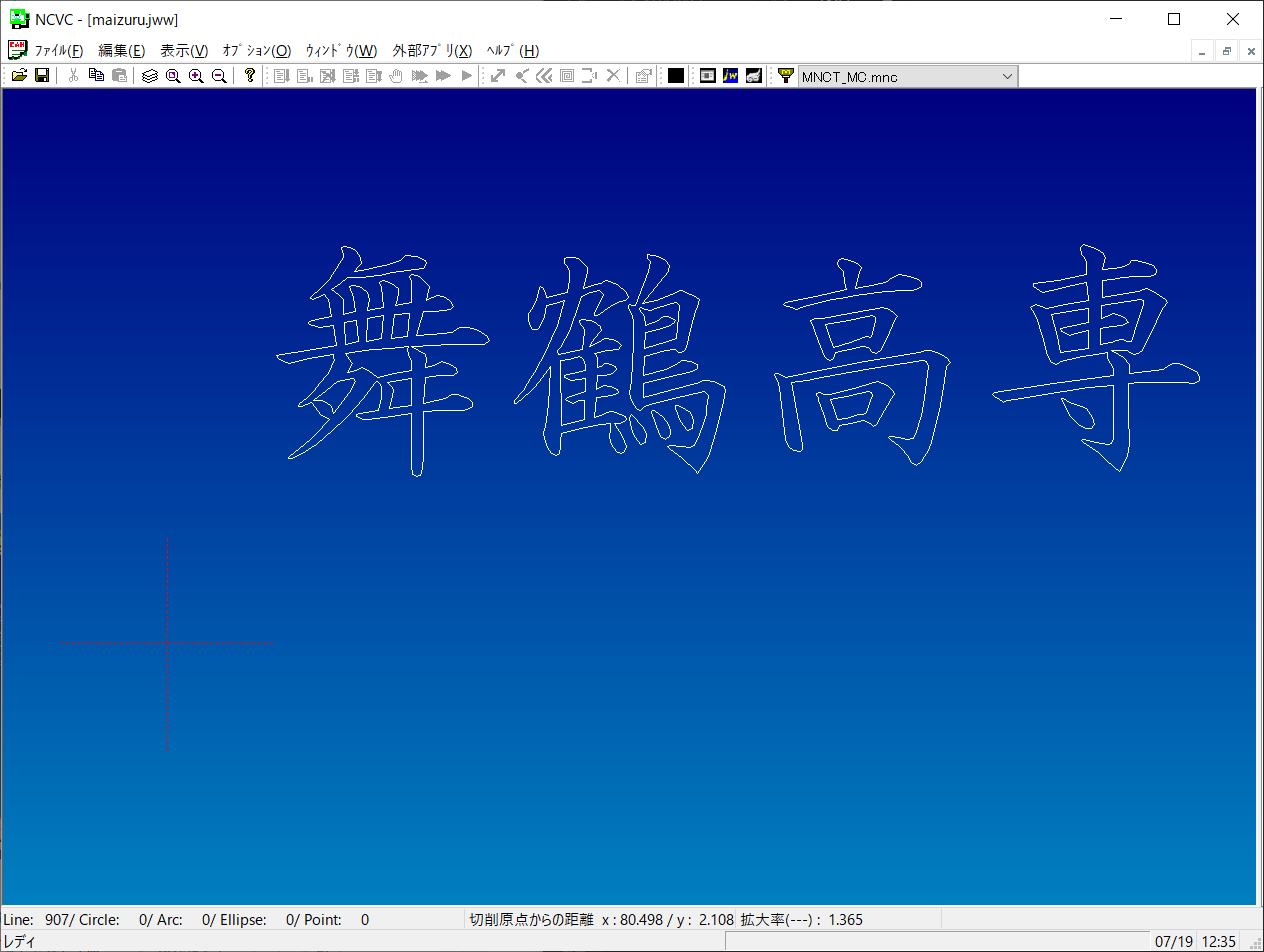
\includegraphics[scale=0.55]{No1/fig/maizuru1.png}
\caption{CADデータの読み込み}
\label{fig:maizuru1.png}
\end{figure}

\subsection{形状認識処理}
 \menu{編集>加工指示>形状認識処理(Ctrl+E)} を選択します.
すると図\ref{fig:maizuru2.png} のようにウィンドウの右側に連続線の図形集合が追加されます。
図形の輪郭が設定できるのは[輪郭集合]に属する図形集合のみです。
それに属する条件は、『交点がなく閉ループの連続線』なので、
CAD側で調整するか、NCVCで図形の分離を行ってください。
詳細は『いまからはじめるNC工作』を参照。

\begin{figure}[H]
\centering
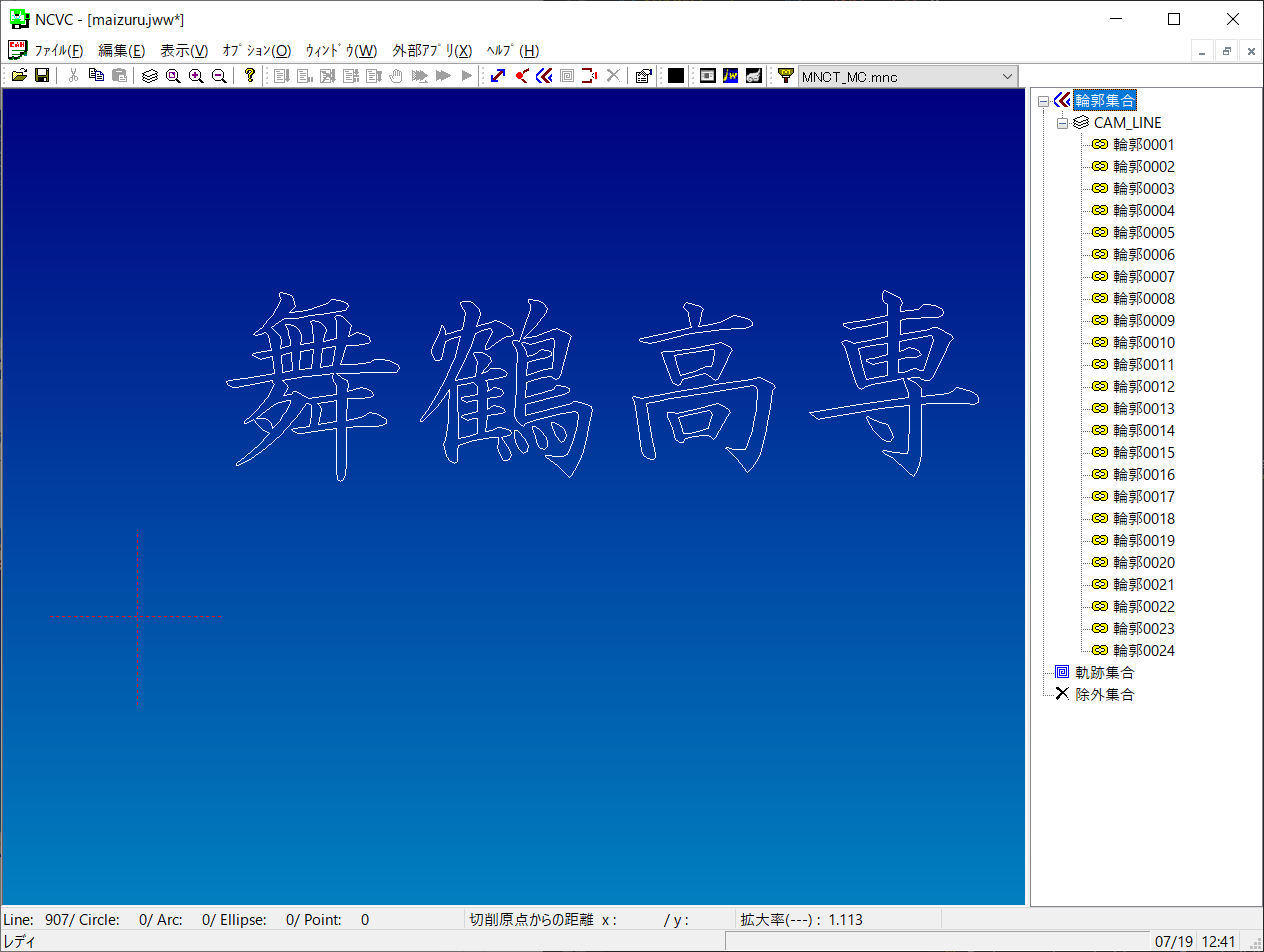
\includegraphics[scale=0.55]{No1/fig/maizuru2.png}
\caption{形状認識処理}
\label{fig:maizuru2.png}
\end{figure}
